%% Creator: Inkscape inkscape 0.48.4, www.inkscape.org
%% PDF/EPS/PS + LaTeX output extension by Johan Engelen, 2010
%% Accompanies image file 'graphicalModel_temporal.pdf' (pdf, eps, ps)
%%
%% To include the image in your LaTeX document, write
%%   \input{<filename>.pdf_tex}
%%  instead of
%%   \includegraphics{<filename>.pdf}
%% To scale the image, write
%%   \def\svgwidth{<desired width>}
%%   \input{<filename>.pdf_tex}
%%  instead of
%%   \includegraphics[width=<desired width>]{<filename>.pdf}
%%
%% Images with a different path to the parent latex file can
%% be accessed with the `import' package (which may need to be
%% installed) using
%%   \usepackage{import}
%% in the preamble, and then including the image with
%%   \import{<path to file>}{<filename>.pdf_tex}
%% Alternatively, one can specify
%%   \graphicspath{{<path to file>/}}
%% 
%% For more information, please see info/svg-inkscape on CTAN:
%%   http://tug.ctan.org/tex-archive/info/svg-inkscape
%%
\begingroup%
  \makeatletter%
  \providecommand\color[2][]{%
    \errmessage{(Inkscape) Color is used for the text in Inkscape, but the package 'color.sty' is not loaded}%
    \renewcommand\color[2][]{}%
  }%
  \providecommand\transparent[1]{%
    \errmessage{(Inkscape) Transparency is used (non-zero) for the text in Inkscape, but the package 'transparent.sty' is not loaded}%
    \renewcommand\transparent[1]{}%
  }%
  \providecommand\rotatebox[2]{#2}%
  \ifx\svgwidth\undefined%
    \setlength{\unitlength}{514.815004bp}%
    \ifx\svgscale\undefined%
      \relax%
    \else%
      \setlength{\unitlength}{\unitlength * \real{\svgscale}}%
    \fi%
  \else%
    \setlength{\unitlength}{\svgwidth}%
  \fi%
  \global\let\svgwidth\undefined%
  \global\let\svgscale\undefined%
  \makeatother%
  \begin{picture}(1,0.36762093)%
    \put(0,0){\includegraphics[width=\unitlength]{graphicalModel_temporal.pdf}}%
    \put(0.09547193,0.29665535){\color[rgb]{0,0,0}\makebox(0,0)[lb]{\smash{$U_0$}}}%
    \put(0.09407952,0.15956687){\color[rgb]{0,0,0}\makebox(0,0)[lb]{\smash{$S_0$}}}%
    \put(0.01881458,0.22563278){\color[rgb]{0,0,0}\makebox(0,0)[lb]{\smash{$Z_0$}}}%
    \put(0.31237857,0.29852096){\color[rgb]{0,0,0}\makebox(0,0)[lb]{\smash{$U_1$}}}%
    \put(0.31409408,0.16143247){\color[rgb]{0,0,0}\makebox(0,0)[lb]{\smash{$S_1$}}}%
    \put(0.23882916,0.22749837){\color[rgb]{0,0,0}\makebox(0,0)[lb]{\smash{$Z_1$}}}%
    \put(0.90558919,0.30139354){\color[rgb]{0,0,0}\makebox(0,0)[lb]{\smash{$U_n$}}}%
    \put(0.90419676,0.16430507){\color[rgb]{0,0,0}\makebox(0,0)[lb]{\smash{$S_n$}}}%
    \put(0.82893184,0.23037096){\color[rgb]{0,0,0}\makebox(0,0)[lb]{\smash{$Z_n$}}}%
    \put(0.53050271,0.02213156){\color[rgb]{0,0,0}\makebox(0,0)[lb]{\smash{$S_f$}}}%
    \put(0.53175169,0.29895161){\color[rgb]{0,0,0}\makebox(0,0)[lb]{\smash{$U_2$}}}%
    \put(0.53346717,0.16186314){\color[rgb]{0,0,0}\makebox(0,0)[lb]{\smash{$S_2$}}}%
    \put(0.4582022,0.22792902){\color[rgb]{0,0,0}\makebox(0,0)[lb]{\smash{$Z_2$}}}%
  \end{picture}%
\endgroup%
